% !TeX spellcheck = en_GB 

\chapter{Exercises}
\section{Sheet 0 - Python}

\newpage
\section{Sheet 1}

\subsection{Assignment 1a - Bias of an estimator} 
\dots
\paragraph{Solution:} 
\begin{minipage}{\textwidth}
	\begin{minipage}[b]{0.49\textwidth}
		\begin{figure}[H]
			\centering
			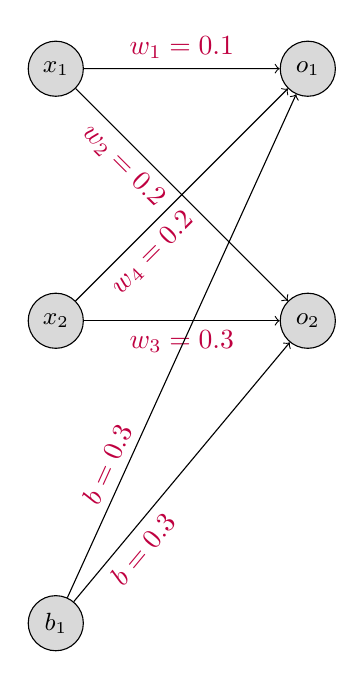
\begin{tikzpicture}[x=2cm,y=2cm] 
			\begin{scope}[scale=1.6]
			
			\tikzstyle{mycircle}=[circle,
			draw=black,
			fill=gray,
			fill opacity = 0.3,
			text opacity=1,
			inner sep=0pt,
			minimum size=7mm,
			font=\small
			]
			\tikzstyle{myline}=[-]
			\tikzstyle{myarrow}=[->]
			
			\coordinate (px1) at (-1, 1);
			\coordinate (px2) at (-1, 0);
			\coordinate (pb1) at (-1, -1.2);
			
			\coordinate (po1) at (0, 1);
			\coordinate (po2) at (0, 0);
			
			
			\node[mycircle] (x1) at (px1) {$x_1$};	
			\node[mycircle] (x2) at (px2) {$x_2$};	
			\node[mycircle] (b1) at (pb1) {$b_1$};	
			
			\node[mycircle] (o1) at (po1) {$o_1$};	
			\node[mycircle] (o2) at (po2) {$o_2$};	
			
			\draw[myarrow] (x1) -- node[purple, auto] {$w_1=0.1$} (o1);			
			\draw[myarrow] (x1) -- node[purple, sloped, anchor=x2, below left] {$w_2=0.2$} (o2);
			
			\draw[myarrow] (x2) -- node[purple, below] {$w_3=0.3$} (o2);			
			\draw[myarrow] (x2) -- node[purple, sloped, anchor=x2, below left] {$w_4=0.2$} (o1);
			
			
			\draw[myarrow] (b1) -- node[purple, sloped, above, near start] {$b=0.3$} (o1);
			\draw[myarrow] (b1) -- node[purple, sloped, below, near start] {$b=0.3$} (o2);
			
			\end{scope}
			\end{tikzpicture}
		\end{figure}
		\captionof{figure}{Multi-Layer Perceptron}
		\label{fig:Sheet5Ex1}
	\end{minipage}
	\hfill
	\begin{minipage}[b]{0.49\textwidth}
		\centering
		\begin{tabular}{ |c | c | c | c | c |}
			\hline
			$n$ & $x_1$ & $x_2$ & $p_1$ & $p_2$\\ \hline
			$1$ & $0.1$ & $0.4$ & $0.1$ & $0.9$\\ \hline
			$2$ & $0.8$ & $0.2$ & $0.95$ & $0.05$\\ \hline
			$3$ & $0.6$ & $0.5$ & $0.4$ & $0.6$\\ \hline
			$4$ & $0.3$ & $0.9$ & $0.75$ & $0.25$\\ \hline
			$5$ & $0.3$ & $0.5$ & $0.9$ & $0.1$\\ \hline
		\end{tabular}
		\captionof{table}{Training batch}
	\end{minipage}
\end{minipage}

\begin{algorithm}[H] 
	\caption{Generative Adversarial Networks (GAN)}%\label{alg:GAN}
	\begin{tabbing}
		\textbf{Output:} \= \kill
		\textbf{Input:} \> a discriminator function $D$,\\
		\> a generator function $G$,\\
		\> noise samples $Z$,\\
		\> true samples $X$ (with an underlying data generation distribution $\IP_{\text{data}}[X]$),\\
		\> desired size of mini-batches $m$,\\
		\> a number $k$ of improvement iterations for the discriminator,\\
		\> stopping criterion $T_{\text{condition}}$\\
		\textbf{Output:} \> a generator $G$ that is able to fool the trained discriminator $D$
	\end{tabbing}
	\begin{algorithmic}[1]
		\While {not $T_{\text{condition}}(f, \theta)$}
		\For {$k$ steps}
		\State Sample a minibatch of noise samples $\{z^{(1)}, \dots, z^{(m)}\}$
		\State Sample a minibatch of true samples $\{x^{(1)}, \dots, x^{(m)}\}$
		\State Perform stochastic gradient ascend for the discriminator:
		\[ \nabla_{\theta^{(d)}}\frac{1}{m}\sum\limits_{i=1}^{m}\Big( \log\big( d(x^{(i)};\theta^{(d)}) \big) + \log\big(1-d\big(g(z^{(i)};\theta^{(g)}),\theta^{(d)}\big)\big) \Big) \]
		\EndFor
		\State Sample a minibatch of noise samples $\{z^{(1)}, \dots, z^{(m)}\}$
		\State Perform stochastic gradient descending for the generator:
		\[ \nabla_{\theta^{(g)}}\frac{1}{m}\sum\limits_{i=1}^{m}\Big(  \log\big(1-d\big(g(z^{(i)};\theta^{(g)}),\theta^{(d)}\big)\big) \Big) \]
		\EndWhile
	\end{algorithmic}	
\end{algorithm}